\RequirePackage{luatex85}
\PassOptionsToPackage{unicode}{hyperref}
\PassOptionsToPackage{naturalnames}{hyperref}
\documentclass{article}
\usepackage{geometry}
\usepackage[cm]{fullpage}
\usepackage{parskip}
\usepackage{physics}
\usepackage{amsmath}
\usepackage{amssymb}
\usepackage[dvipsnames]{xcolor}
\usepackage[colorlinks,linkcolor=blue,citecolor=green]{hyperref}
\usepackage{array}
\usepackage{longtable}
\usepackage{multirow}
\usepackage{comment}
\usepackage{graphicx}
\usepackage{cite}
\usepackage{amsfonts}
\usepackage{bm}
\usepackage{slashed}
\usepackage{dsfont}
\usepackage{mathtools}
\usepackage[compat=1.1.0]{tikz-feynman}
\usepackage{pgfplots}
\pgfplotsset{compat=newest}
\usepackage{simpler-wick} 
\usepackage{mathrsfs}
\usepackage{xparse}
\usepackage{enumerate}
\usepackage{extarrows}
\usepackage[caption=false]{subfig}
% ==============================================================================
% Endnotes
% ==============================================================================
\usepackage{enotez}
% HOWTO: 
% \endnote{}
% Print the notes by adding the following to the end of the document: 
% \printendnotes

% ==============================================================================
% Minted
% ==============================================================================
\usepackage{minted}
\usemintedstyle{colorful}

% ==============================================================================
% Changes: comments and highlights
% ==============================================================================
\let\comment\undefined
\usepackage[highlightmarkup=uwave]{changes}

\allowdisplaybreaks

% ==============================================================================
% mathtools
% ==============================================================================
\newcommand\MTkillspecial[1]{% helper macro
	\bgroup
	\catcode`\&=9
	\let\\\relax%
	\scantokens{#1}%
	\egroup
	}
\DeclarePairedDelimiter\BraceM\{\}
\reDeclarePairedDelimiterInnerWrapper\BraceM{star}{
	\mathopen{#1\vphantom{\MTkillspecial{#2}}\kern-\nulldelimiterspace\right.}
	#2
	\mathclose{\left.\kern-\nulldelimiterspace\vphantom{\MTkillspecial{#2}}#3}
	}
\DeclarePairedDelimiter\bracketM{[}{]}
\reDeclarePairedDelimiterInnerWrapper\bracketM{star}{
	\mathopen{#1\vphantom{\MTkillspecial{#2}}\kern-\nulldelimiterspace\right.}
	#2
	\mathclose{\left.\kern-\nulldelimiterspace\vphantom{\MTkillspecial{#2}}#3}
	}
\let\Bqty\relax
\let\bqty\relax
\newcommand{\Bqty}[1]{\BraceM*{#1}}
\newcommand{\bqty}[1]{\bracketM*{#1}}
\DeclarePairedDelimiter\ceil{\lceil}{\rceil}
\DeclarePairedDelimiter\floor{\lfloor}{\rfloor}

% ==============================================================================
% ifthen for User-definition
% ==============================================================================
\usepackage{ifthen}
% HOWTO:
% \ifthenelse{<test>}{<code for true>}{<code for false>}

% ==============================================================================
% User Definition
% ==============================================================================
\newcommand{\red}[1]{{\color{red}#1}}
\newcommand{\mm}[1]{\frac{\dd^4#1}{(2\pi)^4}}
\newcommand{\mme}[1]{\frac{\dd^3\vb{#1}}{(2\pi)^3}}
\newcommand{\mmd}[2][d]{\ifthenelse{\equal{#1}{1}}{\frac{\dd {#2}}{2\pi}}{\frac{\dd^{#1}{#2}}{(2\pi)^{#1}}}}

\newcommand{\glprog}[2]{\int\frac{\dd #1}{2\pi}\frac{ie^{-i#1 #2}}{#1+i\epsilon}}

\makeatletter
\newcommand{\pushright}[1]{\ifmeasuring@#1\else\omit\hfill$\displaystyle#1$\fi\ignorespaces}
\newcommand{\pushleft}[1]{\ifmeasuring@#1\else\omit$\displaystyle#1$\hfill\fi\ignorespaces}
\makeatother

\NewDocumentCommand\NL{s}{%
  \IfBooleanTF#1%
    {\notag\\\times}% If a star is seen
    {\notag\\}%     If no star is seen
}



% ==============================================================================
% Tikz-Feynman Externalization
% ==============================================================================
\usepackage{shellesc}
\usetikzlibrary{external}
% \usepgfplotslibrary{external}
\tikzexternalize[shell escape=-enable-write18,prefix=./QuasiPDF1LRes/,system call={lualatex \tikzexternalcheckshellescape -halt-on-error -interaction=batchmode -jobname "\image" "\texsource"},up to date check=diff]

\tikzfeynmanset{
	Eikonal/.style={
		/tikz/draw=none,
		/tikz/decoration={name=none},
		/tikz/postaction={
			/tikz/draw,
			/tikz/double distance=2pt,
			% /tikzfeynman/with arrow=0.5,
		},
	},
	half right/.append style={
		/tikz/looseness=2
	},
	half left/.append style={
		/tikz/looseness=2
	}
}

% ==============================================================================
% Tikz-Feynman Auxiliary
% ==============================================================================
\def\FDWidth{3cm}
\def\FDHeight{3cm}
\def\FDWidthS{2cm}
\def\FDHeightS{2cm}


\newcommand{\WN}[1]{\textcolor{RawSienna}{#1}}
\newcommand{\CJ}[1]{\textcolor{RoyalBlue}{#1}}


\title{One Loop Matching for Quasi PDF}
\author{Yingsheng Huang}
\begin{document}
\maketitle
\clearpage
\section{Diagrams}
\begin{figure}[!htpb]
	\centering\null
	\hfil\subfloat[8]{
		\centering
		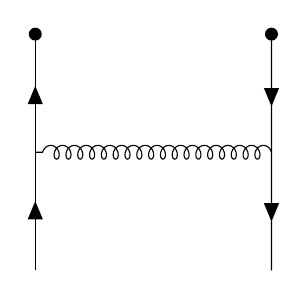
\begin{tikzpicture}[baseline=($(a)!0.5!(exa)$.base)]
			\begin{feynman}
				\node[dot] (a);
				\node[right=\FDWidth of a,dot] (b);open
				\vertex[below=\FDHeight of a] (exa);
				\vertex[below=\FDHeight of b] (exb);
				\vertex at ($(exa)!0.5!(a)$) (a1);
				\vertex at ($(exb)!0.5!(b)$) (b1);
				\diagram*{
				% (a) --[Eikonal] (b);
				(exa) --[fermion] (a1) --[fermion] (a);
				(b) --[fermion] (b1) --[fermion] (exb);
				(b1) --[gluon] (a1);
				};
			\end{feynman}
		\end{tikzpicture}
		\label{2:--}
	}\hfil
	\subfloat[4]{
		\centering
		\begin{tikzpicture}[baseline=($(a)!0.5!(exa)$.base)]
			\begin{feynman}
				\node[dot] (a);
				\node[right=\FDWidth of a,dot] (b);
				\vertex at ($(a)!0.5!(b)$) (o);
				\vertex[below=\FDHeight of a] (exa);
				\vertex[below=\FDHeight of b] (exb);
				\vertex at ($(exa)!0.5!(a)$) (a1);
				\vertex at ($(exb)!0.5!(b)$) (b1);
				\diagram*{
				(o) --[Eikonal] (b);
				(exa) --[fermion] (a1) --[fermion] (a);
				(b) --[fermion] (exb);
				(a1) --[gluon] (o);
				};
			\end{feynman}
		\end{tikzpicture}
		\label{2/-}
	}\hfil
	\subfloat[3]{
		\centering
		\begin{tikzpicture}[baseline=($(a)!0.5!(exa)$.base)]
			\begin{feynman}
				\node[dot] (a);
				\node[right=\FDWidth of a,dot] (b);
				\vertex at ($(a)!0.5!(b)$) (o);
				\vertex[below=\FDHeight of a] (exa);
				\vertex[below=\FDHeight of b] (exb);
				\vertex at ($(exa)!0.5!(a)$) (a1);
				\vertex at ($(exb)!0.5!(b)$) (b1);
				\diagram*{
				(a) --[Eikonal] (o);
				(exa) --[fermion] (a);
				(b) --[fermion] (b1) --[fermion] (exb);
				(b1) --[gluon] (o);
				};
			\end{feynman}
		\end{tikzpicture}
		\label{2-`}
	}\hfil
	\subfloat[5]{
		\centering
		\begin{tikzpicture}[baseline=($(a)!0.5!(exa)$.base)]
			\begin{feynman}
				\node[dot] (a);
				\node[right=\FDWidth of a,dot] (b);
				\vertex at ($(a)!0.3!(b)$) (o1);
				\vertex at ($(a)!0.7!(b)$) (o2);
				\vertex[below=\FDHeight of a] (exa);
				\vertex[below=\FDHeight of b] (exb);
				\diagram*{
				(a) --[Eikonal] (o1);
				(b) --[Eikonal] (o2);
				(exa) --[fermion] (a);
				(b) --[fermion] (exb);
				(o1) --[gluon, half right] (o2);
				};
			\end{feynman}
		\end{tikzpicture}
		\label{2-v-}
	}\hfil\null\\\null\hfil
	\subfloat[1]{
		\centering
		\begin{tikzpicture}[baseline=($(a)!0.5!(exa)$.base)]
			\begin{feynman}
				\node[dot] (a);
				\node[right=\FDWidth of a,dot] (b);
				\vertex at ($(a)!0.5!(b)$) (o);
				\vertex[below=\FDHeight of a] (exa);
				\vertex[below=\FDHeight of b] (exb);
				\vertex at ($(exa)!0.5!(a)$) (a1);
				\vertex at ($(exb)!0.5!(b)$) (b1);
				\diagram*{
				(o) --[Eikonal] (a);
				(exa) --[fermion] (a1) --[fermion] (a);
				(b) --[fermion] (exb);
				(a1) --[gluon] (o);
				};
			\end{feynman}
		\end{tikzpicture}
		\label{2-/}
	}\hfil
	\subfloat[7]{
		\centering
		\begin{tikzpicture}[baseline=($(a)!0.5!(exa)$.base)]
			\begin{feynman}
				\node[dot] (a);
				\node[right=\FDWidth of a,dot] (b);
				\vertex at ($(a)!0.5!(b)$) (o);
				\vertex[below=\FDHeight of a] (exa);
				\vertex[below=\FDHeight of b] (exb);
				\vertex at ($(exa)!0.5!(a)$) (a1);
				\vertex at ($(exb)!0.5!(b)$) (b1);
				\diagram*{
				(b) --[Eikonal] (o);
				(exa) --[fermion] (a);
				(b) --[fermion] (b1) --[fermion] (exb);
				(b1) --[gluon] (o);
				};
			\end{feynman}
		\end{tikzpicture}
		\label{2`-}
	}\hfil
	\subfloat[2]{
		\centering
		\begin{tikzpicture}[baseline=($(a)!0.5!(exa)$.base)]
			\begin{feynman}
				\node[dot] (a);
				\node[right=\FDWidth of a,dot] (b);
				\vertex at ($(a)!0.5!(b)$) (o);
				\vertex at ($(a)!0.2!(b)$) (o1);
				\vertex at ($(a)!0.8!(b)$) (o2);
				\vertex[below=\FDHeight of a] (exa);
				\vertex[below=\FDHeight of b] (exb);
				\diagram*{
				(a) --[Eikonal] (o);
				(exa) --[fermion] (a);
				(b) --[fermion] (exb);
				(o1) --[gluon, half right] (o);
				};
			\end{feynman}
		\end{tikzpicture}
		\label{2-o}
	}\hfil
	\subfloat[6]{
		\centering
		\begin{tikzpicture}[baseline=($(a)!0.5!(exa)$.base)]
			\begin{feynman}
				\node[dot] (a);
				\node[right=\FDWidth of a,dot] (b);
				\vertex at ($(a)!0.5!(b)$) (o);
				\vertex at ($(a)!0.2!(b)$) (o1);
				\vertex at ($(a)!0.8!(b)$) (o2);
				\vertex[below=\FDHeight of a] (exa);
				\vertex[below=\FDHeight of b] (exb);
				\diagram*{
				(b) --[Eikonal] (o);
				(exa) --[fermion] (a);
				(b) --[fermion] (exb);
				(o) --[gluon, half right] (o2);
				};
			\end{feynman}
		\end{tikzpicture}
		\label{2o-}
	}\hfil\null
	\caption{Diagrams of quasi PDF in Feynman gauge. }
\end{figure}

\section{Analytic Results}
\begin{align}
    &\Gamma_a=\tilde{q}_{11}=\frac{\alpha_{S} C_{F}}{2 \pi}\left\{\begin{array}{cc}
        {(x-1) \ln \frac{x-1}{x}+1,} & {x>1} \\
        {(1-x) \ln \frac{\left(P^{z}\right)^{2}}{m^{2}}+(1-x) \ln \frac{4 x}{1-x}+1-\frac{2 x}{1-x},} & {0<x<1} \\
        {(x-1) \ln \frac{x}{x-1}-1,} & {x<0}
        \end{array}\right.\\
    &\Gamma_b=\tilde{q}_{12}=\frac{\alpha_{S} C_{F}}{2 \pi}\left\{\begin{array}{ll}
        {-\frac{2 x}{1-x} \ln \frac{x-1}{x}-\frac{1}{1-x},} & {x>1} \\
        {\frac{2 x}{1-x} \ln \frac{\left(p^{z}\right)^{2}}{m^{2}}+\frac{2 x}{1-x} \ln \frac{4 x}{1-x}+1-\frac{x}{1-x},} & {0<x<1} \\
        {-\frac{2 x}{1-x} \ln \frac{x}{x-1}+\frac{1}{1-x},} & {x<0}
        \end{array}\right.\\
    &\Gamma_d=\tilde{q}_{13}=\frac{\alpha_{S} C_{F}}{2 \pi}\left\{\begin{array}{ll}
        {\frac{1}{1-x},} & {x>1} \\
        {-\frac{1}{1-x},} & {0<x<1} \\
        {-\frac{1}{1-x},} & {x<0}
        \end{array}\right.
\end{align}

\section{Numerical Results ($z=1/4$)}
\paragraph{Diagram a/8}
\begin{minted}[breaklines]{mathematica}
    0.349565 CV(1,3) CV(2,4/3)-0.477465 CV(1,3) CV(2,4/3) log(s)
\end{minted}
\paragraph{Diagram b/4}
\begin{minted}[breaklines]{mathematica}
    0.212207 CV(1,3) CV(2,4/3) log(s)-0.273255 CV(1,3) CV(2,4/3)
\end{minted}
\paragraph{\CJ{Diagram c/3}}
\begin{minted}[breaklines]{mathematica}
    0.212207 CV(1,3) CV(2,4/3) log(s)-0.273255 CV(1,3) CV(2,4/3)
\end{minted}
\paragraph{Diagram d/5}
\begin{minted}[breaklines]{mathematica}
    (-0.8488263632 +- 0)*CV(1,3)*CV(2,4/3)
\end{minted}
\paragraph{Diagram e/1}
\begin{minted}[breaklines]{c}
	-(pow(ep, -1)*VE(0.0008169409107633463681570624056631273862747042526785892777191`57.91219064520137, 1.573559789424925624931668641423792657070683730085710006430199999999999999999996`58.1968832491393*^-37)) - I*Log(s)*VE(0.001710997042447389198192130544519783670764184528834537099249`57.23324925883983, 4.271482028579777382697383004256461656538920523665798674249`57.63057858349424*^-39) + Log(s)*VE(0.0020113886808464843453169828119028634461644104203568234504405`58.303496001793235, 1.7236940063183554104424057773355075936432380125625874075805`58.23646017148736*^-39) + I*VE(0.002041472822019871261757020507759581691885328968064951861992`57.309943602566456, 7.62407758243823923660715590987450803330247834778547289629`56.88218730702342*^-7) - VE(0.008867290012058965928678591934196724392569718269407575616033`57.947790912657496, 7.243789259153541902289364987292676931611449905233727976407`57.85996580705919*^-7)
\end{minted}
\paragraph{Diagram f/7}
\begin{minted}[breaklines]{c}
	-(pow(ep, -1)*VE(0.000816940910763346368157062405663127281012571570463568865045`56.91219064520138, 9.160798889579999167228752424173255626841843784041611172283`57.961933349018004*^-45)) + I*Log(s)*VE(0.0017109970424473891981921305445197823837827362823448366985874`58.23324925883983, 1.0475436352060500030082253984993710859395727446288236243772`58.02017212245887*^-44) + Log(s)*VE(0.00201138868084648434531698281190286331272082601494039124093`56.30349600179324, 6.477663009490828372139324135250424049035023383857992870721`57.81141835075576*^-45) - I*VE(0.0020414712973779882625571858127674160994923607132845858070926`58.30994327822033, 6.135943024985027649893213265102755089734278511599157336027`57.787881318338336*^-10) - VE(0.008867290504621969964938003672921487677952902455900176633184`57.94779093678183, 4.82755896183491993338063389951537847303460832348703277903`56.68372758677938*^-10)
\end{minted}
\end{document}